\documentclass{emulateapj}
%\documentclass[12pt,preprint]{aastex}

\usepackage{graphicx}
\usepackage{float}
\usepackage{amsmath}
\usepackage{epsfig,floatflt}
\usepackage{fourier}

\DeclareMathAlphabet{\mathcal}{OMS}{cmsy}{m}{n}
\SetMathAlphabet{\mathcal}{bold}{OMS}{cmsy}{b}{n}


\begin{document}

\title{Project 1}

\author{Stig-Nicolai Foyn, Christer Dreierstad}

\email{stignicf@student.matnat.uio.no, chrisdre@student.matnat.uio.no}

\altaffiltext{1}{Institute of physics, University of
  Oslo, P.O.\ Box 1029 Blindern, N-0315 Oslo, Norway}


%\date{Received - / Accepted -}

\begin{abstract}
Comparing general and tailored methods for solving second order differential equations this study will present that producing a specialized method reduces the run time of a numerical solver without losing numerical accuracy. Reducing the floating point operations (FLOPS) will be proven efficient for large scale calculations.

  %State problem. Briefly describe method and data. Summarize main results.
\end{abstract}
\keywords{computational science --- numerical methods: error estimation, run time --- methods: numerical, tridiagonal matrices}

\section{Introduction}
\label{sec:introduction}
This study on generalized and tailored numerical algorithms will focus on how a differential equation is solved numerically most efficiently while not reducing the accuracy of the calculations. By comparing the run time and observing the numerical error of the calculations . To specify, the equation in question is the one dimensional Poisson equation:
%
\begin{equation*}
    {\nabla^{2}} \Phi = -4\pi \rho(r),
\end{equation*}
%
where $\Phi$ is the electrostatic potential generated by a localized charge distribution and $\rho$ is the charge density. This equation is used in electromagnetism, but in this case it was only necessary to analyze a normalized equation on the same form. Our normalized one dimensional Poisson equation can then be written as:
%
\begin{equation}\label{eq:-u''}
    -\frac{du^2}{dx^2} = f(x).
\end{equation}

Further rewriting this as a set of linear equation will allow us to solve it using our numerical algorithms.

%Discuss background, physical importance and possibly some history of
%the problem that is being studied in this paper.


\section{Method}
\label{sec:method}
For the study we consider a solution for the source term $f(x)$ to be
%
\begin{gather*}\label{eq:f(x)}
    f(x) = 100e^{-10x},
\end{gather*}
%
which has a closed form solution 
%
\begin{gather}\label{eq:u(x)}
u(x) = 1-(1-e^{10})x-e^{-10x},
\end{gather}
%
which yields $-f(x)$ when taking the second derivative. 

We consider the one dimensional Poisson equation to uphold Dirichlet boundary conditions; $u(0)=u(1)=0$, so $x \in [0,1]$. The second order derivative $u(x)$ can be represented as
%
\begin{gather}\label{eq:du/dx}
 -\frac{du^2}{dx^2} = -\left(\frac{u(x+h) + u(x-h) - 2u(x)}{h^2} + \mathcal{O}(h^2)\right),
\end{gather}
%
where h is the step size. 

\subsection{Numerical representation}
By approximating equation \eqref{eq:du/dx} and discretizing over x we get
%
\begin{gather*}
    -\frac{du^2}{dx^2} = -\frac{u_{i+1} + u_{i-1} - 2u_i}{h^2} = f(x_i) = f_i.
\end{gather*}
%
To simplify the calculations and reduce the FLOPS, we multiply the above equation by $h^2$ and rewrite $f'_i = h^2f_i = h^2 100 e^{-10x_i}$, such that the final discretized equation for solving equation \eqref{eq:-u''} is
%
\begin{gather}\label{eq:u_discretized}
    -\left(u_{i-1} - 2u_i + u_{i+1}\right) = f'_i.
\end{gather}
%
The linear combination above can be represented by a matrix vector multiplication. The matrix will consist of the coefficients of the $u_i$'s along the central, upper and lower diagonal, making up a tridiagonal matrix. The coefficient, after taking the outer sign into  consideration, are -1, 2 and -1 respectively. The vector will consist of the values of the $u_i$'s. The matrix representation will therefore be on the following form:
%
\[ \boldsymbol{Au} =
\begin{array}{c}
\begin{bmatrix}\label{eq:Au=f}
b_1     & c_1           & 0         & \dots     & \dots     & 0 \\
a_1     & b_2           & c_2       & 0         & \dots     & \dots \\
0       & a_2           & b_3       & c_3       & 0     & \dots\\
\dots  &  0            & a_3       & b_4       & \dots    & 0 \\
\dots  & \dots        & 0 & \dots    & \dots    & c_{n-1} \\
0       & \dots         & \dots         & 0         & a_{n-1}   & b_n   \\
\end{bmatrix}
\begin{bmatrix}
u_1 \\
u_2 \\
\dots \\
\dots \\
\dots \\
u_n
\end{bmatrix}
=
\begin{bmatrix}
f'_1 \\
f_2 \\
\dots \\
\dots \\
\dots \\
f'_n
\end{bmatrix}
\end{array}
= \boldsymbol{f'_i}.
\]
%
Since we are considering fixed end points for $u$ we do not include $i = 0$ and $i = n+1$ in the calculations for updating the $u_i$'s.
%\begin{bmatrix}
%\Tilde{f}_1 \\
%\Tilde{f}_2 \\
%\dots \\
%\dots \\
%\dots \\
%\Tilde{f}_n
%\end{bmatrix}
%\end{array}


\subsection{Specific algorithm}

\subsection{Armadillo}

%Summarize properties of data. Which data are used (experiment,frequencies etc.)? Pixel resolution ($N_{\textrm{side}}$),$\ell_{\textrm{max}}$ -- everything necessary to repeat the analysisfor other researchers.

\section{Results}
\label{sec:results}
\subsection{Numerical error}


\begin{figure}[H]
    \centering
    \includegraphics[size=0.25\textwidth]{p1bplot.png}
    \caption{The solution of the differential equation using a generalized algorithm, the three different plots show the $nxn$ matrix with $n=10$, $n=100$, $n=1000$ }
    \label{fig1: Generalized algorithm}
\end{figure}

\begin{figure}[H]
    \centering
    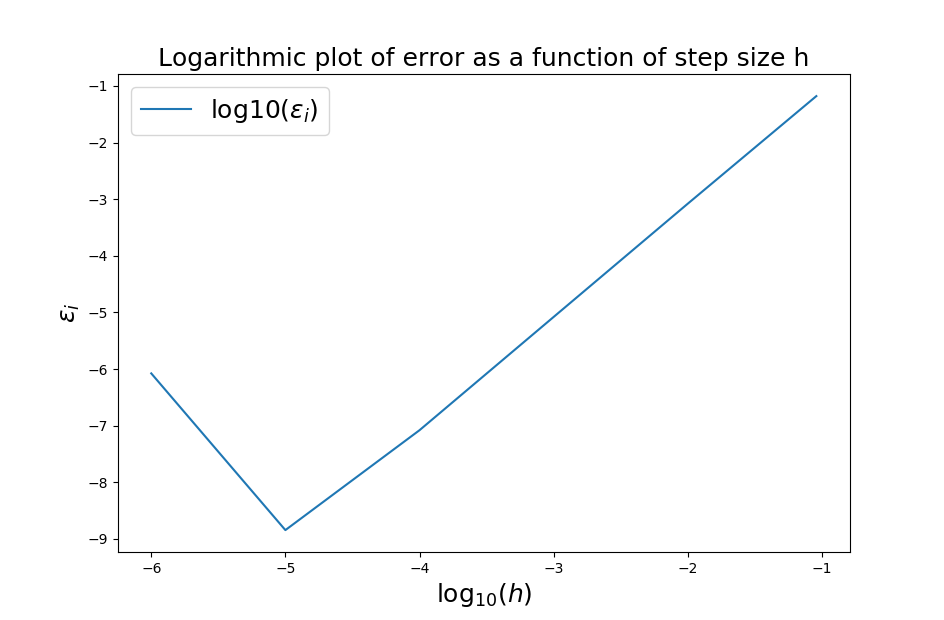
\includegraphics[size=0.25\textwidth]{plot1d.png}
    \caption{}
    \label{fig1:1d}
\end{figure}

\subsection{Program CPU time}
\begin{deluxetable}{lccc}
%\tablewidth{0pt}
\tablecaption{\label{tab:results}}
\tablecomments{This table contains average CPU times for all the algorithms}
\tablecolumns{4}
\tablehead{Column 1  & Column 2 & Column 3 & Column 4}
\startdata
Item 1 & Item 2 & Item 3 & Item 4
\enddata
\end{deluxetable}

\section{Conclusions}
\label{sec:conclusions}

%Summarize results. Discuss their importance, referring to the discovery to the initial seeds for structure formation. Mention that these results are in good agreement with expectations from inflationary theory.



%\begin{figure}[t]
%
%\mbox{\epsfig{figure=filename.eps,width=\linewidth,clip=}}
%
%\caption{Description of figure -- explain all elements, but do not
%draw conclusions here.}
%\label{fig:figure_label}
%\end{figure}



\begin{deluxetable}{lccc}
%\tablewidth{0pt}
\tablecaption{\label{tab:results}}
\tablecomments{Summary of main results.}
\tablecolumns{4}
\tablehead{Column 1  & Column 2 & Column 3 & Column 4}
\startdata
Item 1 & Item 2 & Item 3 & Item 4
\enddata
\end{deluxetable}



\begin{acknowledgements}

\end{acknowledgements}

\begin{thebibliography}{}

\bibitem[G{\'o}rski et al.(1994)]{gorski:1994} G{\'o}rski, K. M.,
  Hinshaw, G., Banday, A. J., Bennett, C. L., Wright, E. L., Kogut,
  A., Smoot, G. F., and Lubin, P.\ 1994, ApJL, 430, 89

\end{thebibliography}


\end{document}
